\documentclass[tikz,border=2pt]{standalone}
\usepackage{amsmath,amssymb}
\usepackage{pgfplots}
\pgfplotsset{compat=1.18}

\begin{document}
% A fair die: the discrete uniform distribution on {1,...,6}, every value with probability 1/6.
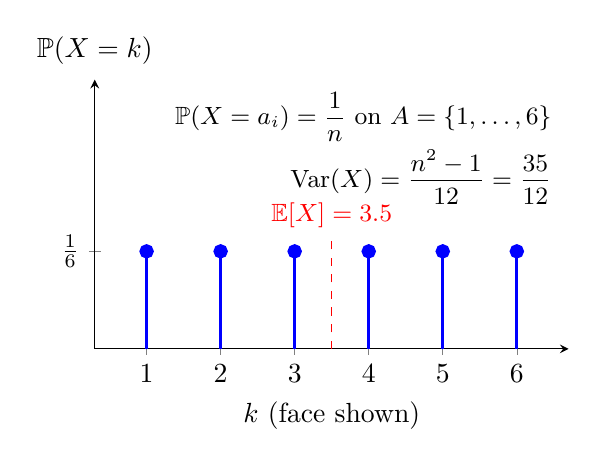
\begin{tikzpicture}
	\begin{axis}[
		axis lines=left, xmin=0.3, xmax=6.7, ymin=0, ymax=0.46,
		xtick={1,...,6}, ytick={0.1667}, yticklabels={$\tfrac16$},
		xlabel={$k$ (face shown)}, ylabel={$\mathbb{P}(X=k)$}, ylabel style={rotate=-90, anchor=south, at={(axis description cs:0,1.02)}},
		width=7.6cm, height=5cm, clip=false
		]
		\addplot[ycomb, blue, very thick, mark=*, mark size=2pt] coordinates {(1,0.1667) (2,0.1667) (3,0.1667) (4,0.1667) (5,0.1667) (6,0.1667)};
		\draw[red, dashed] (axis cs:3.5,0) -- (axis cs:3.5,0.19);
		\node[red, anchor=south, font=\small] at (axis cs:3.5,0.19) {$\mathbb{E}[X]=3.5$};
		\node[anchor=north east, font=\small, align=right] at (axis cs:6.6,0.455) {$\mathbb{P}(X=a_i)=\dfrac1n$ on $A=\{1,\dots,6\}$\\[2pt] $\operatorname{Var}(X)=\dfrac{n^2-1}{12}=\dfrac{35}{12}$};
	\end{axis}
\end{tikzpicture}
\end{document}
